\RequirePackage{lineno}
\documentclass[aps,prl,preprint]{revtex4-1}

\usepackage{amsmath,amssymb,amsfonts}
\usepackage{siunitx}
\sisetup{separate-uncertainty=true}
\usepackage{fancyref}
\usepackage{graphicx}
\usepackage{listings}
\lstset{basicstyle=\ttfamily}
\usepackage{hyperref}
\usepackage[dvipsnames]{xcolor}
\hypersetup{
  colorlinks=true,
  linkcolor=violet,
  urlcolor=blue,
  citecolor=blue}

\begin{document}
\linenumbers
\title{Is momentum conserved?}
\author{\textbf{YOUR NAME}}
\email{lastname\_24@mbs.net}
\author{D Evangelista}
\affiliation{Morristown-Beard School}

\begin{abstract}
Momentum is the product of mass times velocity ($\vec{p}=m\vec{v}$). It is potentially useful for understanding the mechanics of collisions. We examined if momentum is conserved during inelastic collisions using an instrumented, one-dimensional cart system. \textbf{We found... You will write one sentence to finish off the ABSTRACT summarizing what you found.}
\end{abstract}
\maketitle
\section{Introduction}
Momentum is the product of mass times velocity:
\begin{equation}
\text{momentum}\ \vec{p} = m \vec{v},
\label{eq:momentum}
\end{equation}
where $m$ is mass in \si{\kilo\gram} and $\vec{v}$ is the velocity in \si{\meter\per\second} \cite{newton-1687-principia}.  \Fref{eq:momentum} reflects that the ``hitting power'' of an object involves both its mass and its velocity \cite{newton-1687-principia}. Formally, momentum is a vector quantity; here we consider one-dimensional (1D) collisions and will drop the vector notation for simplicity.  

Momentum is potentially useful for understanding collisions in which two bodies collide and stick (as in inelastic collisions) or bounce off one another (as in elastic collisions). If momentum is conserved during such collisions, it could be a powerful and useful concept for quickly and easily determining the final velocities of each of the bodies \cite{newton-1687-principia}. 

Therefore, we wish to answer the question, is momentum conserved? We consider the total momentum of the two-body system before ($p_0$) and after ($p_f$) the collision as
\begin{align}
p_0 &= m_1 v_1 + m_2 v_2\ \text{before collision} \\
p_f &= m_1 v_{1,f} + m_2 v_{2,f}\ \text{after collision}. 
\end{align}
We hypothesize that momentum is conserved during such collisions:
\begin{equation}
H_0: p_f = p_0\ \text{(momentum is conserved)}.
\end{equation}
Alternatively, momentum could somehow increase during a collision; or it could decrease owing to friction or other forces bleeding momentum away: 
\begin{align}
H_1: p_f &> p_0\ \text{(momentum increases)} \\
H_2: p_f &< p_0\ \text{(momentum decreases)} .
\end{align}

We tested these hypotheses by conducting a large number of two-body inelastic collisions with known masses and observing the velocities before and after the collision. For each collision, we found the total system $p_0$ and $p_f$ to determine whether momentum is conserved or not. 
\begin{figure}[h]
\begin{center}
%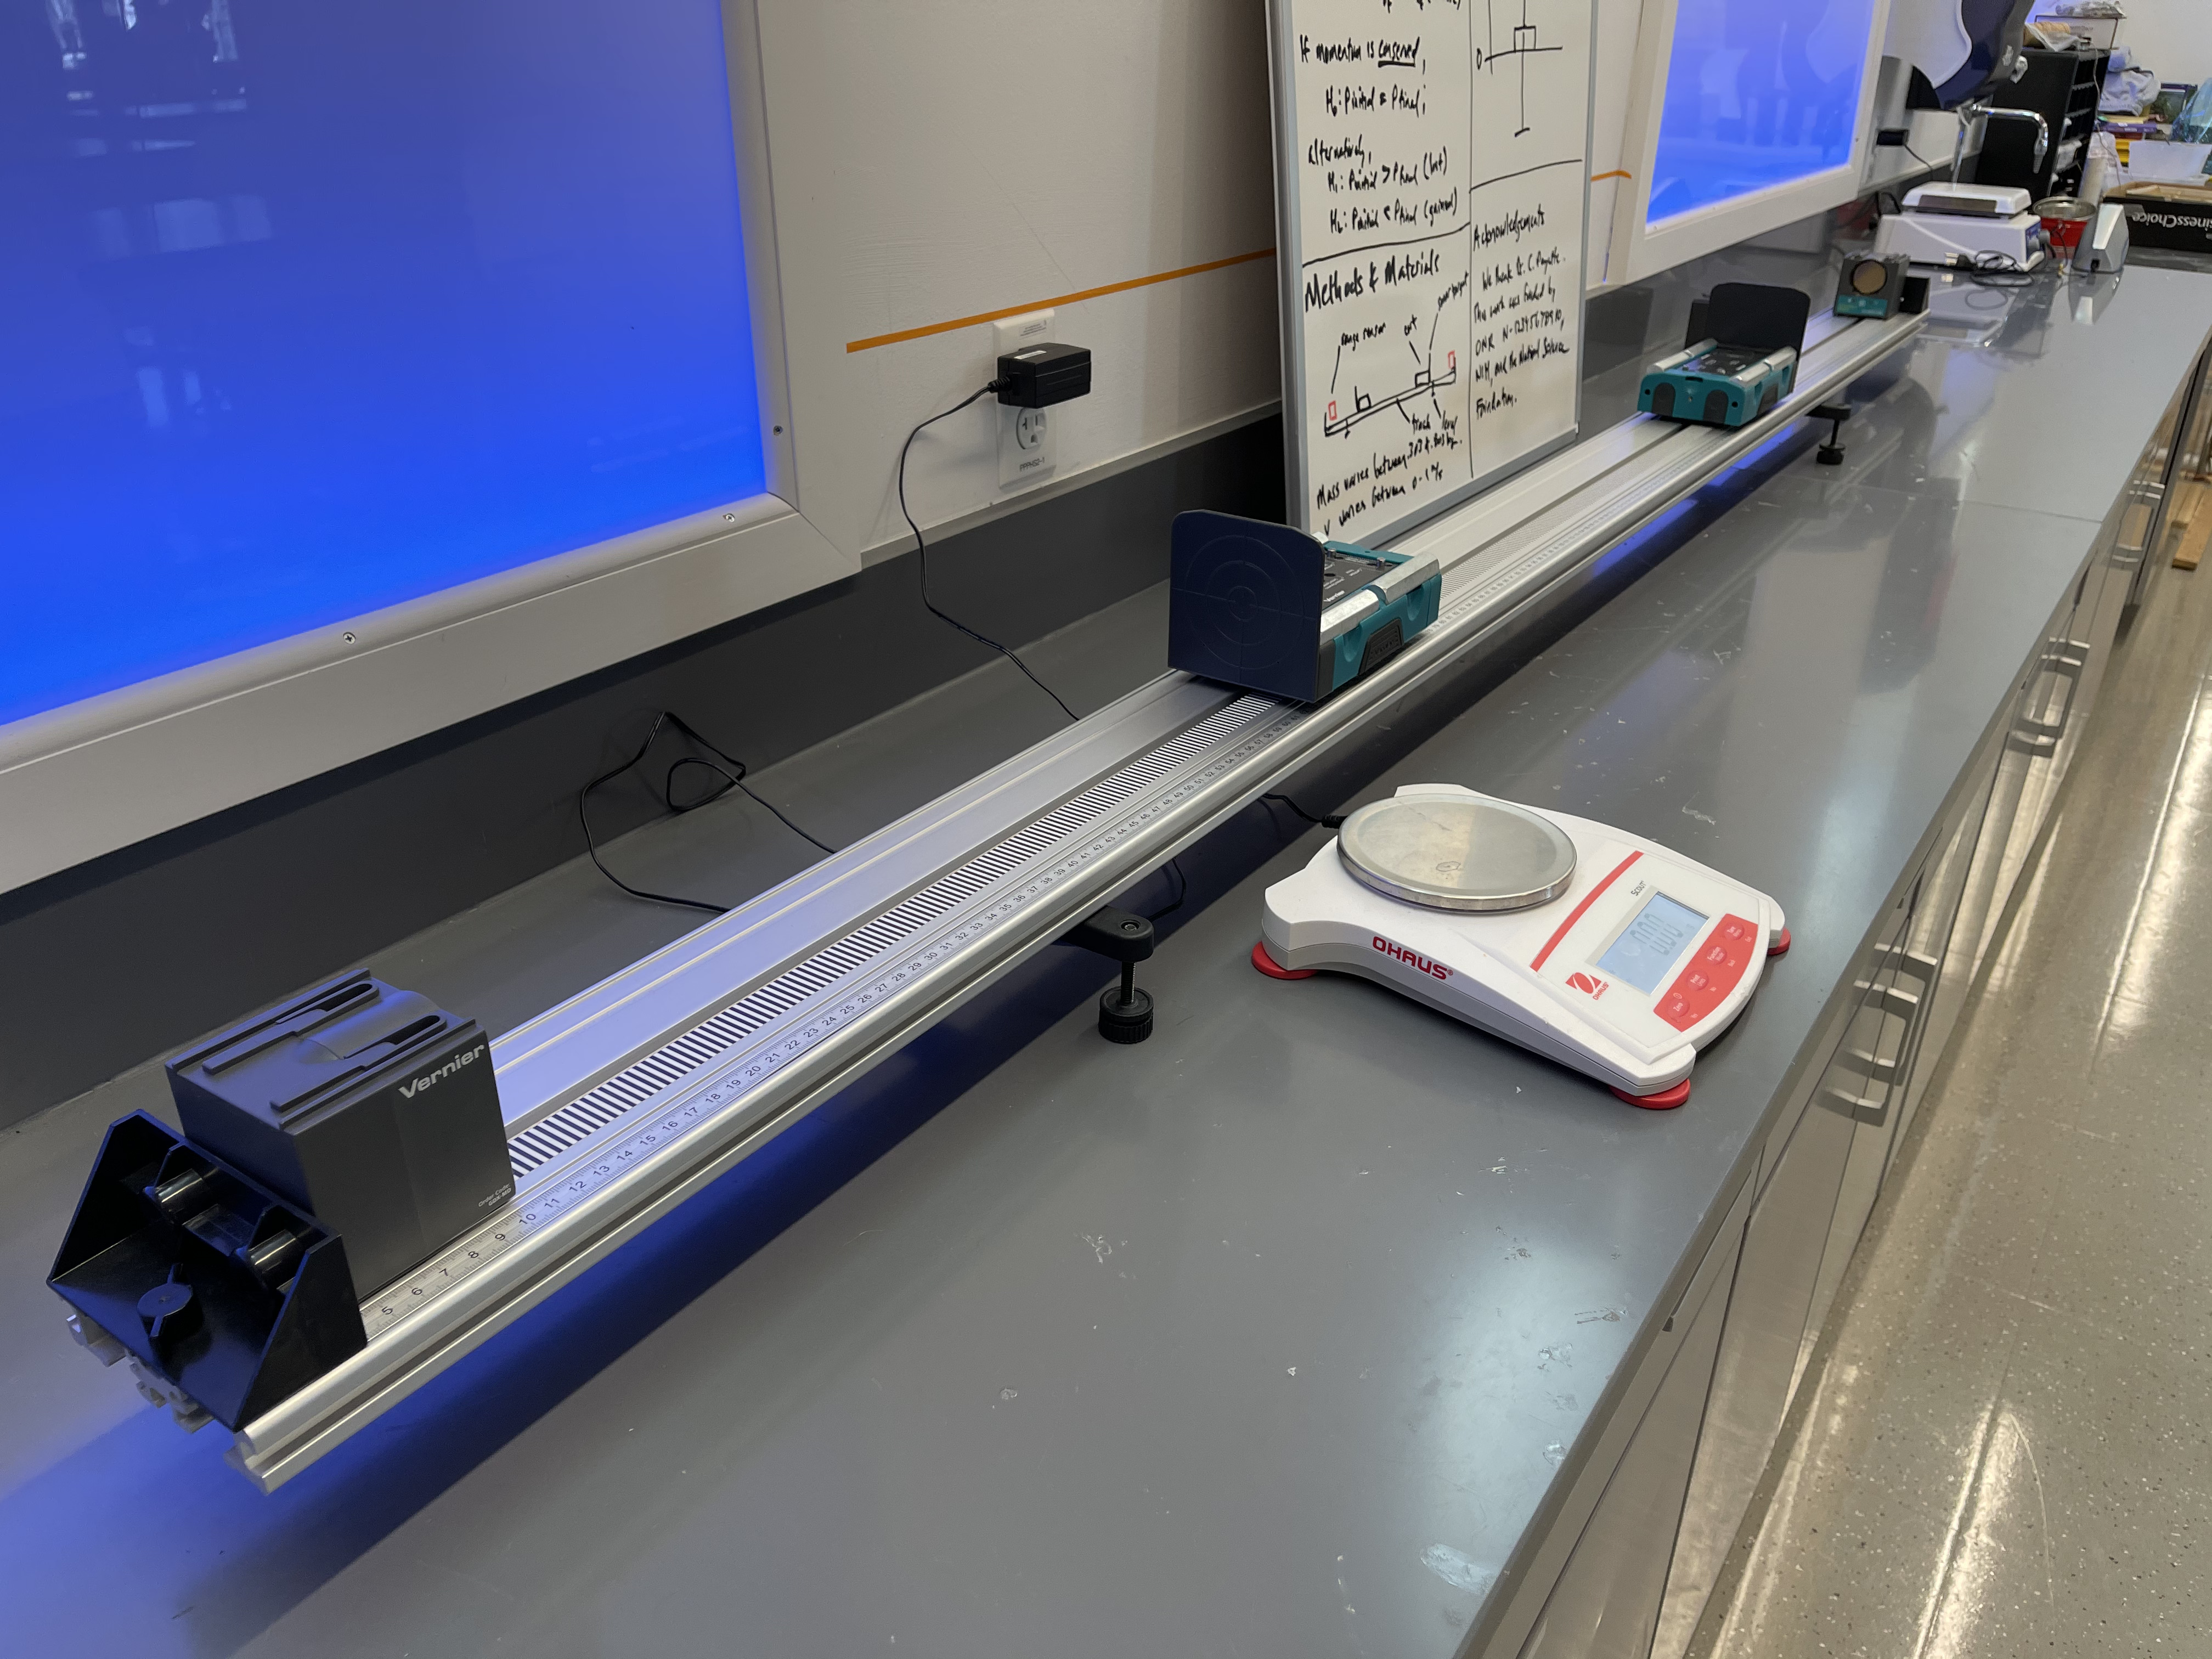
\includegraphics[width=\columnwidth]{IMG_6253.jpg}
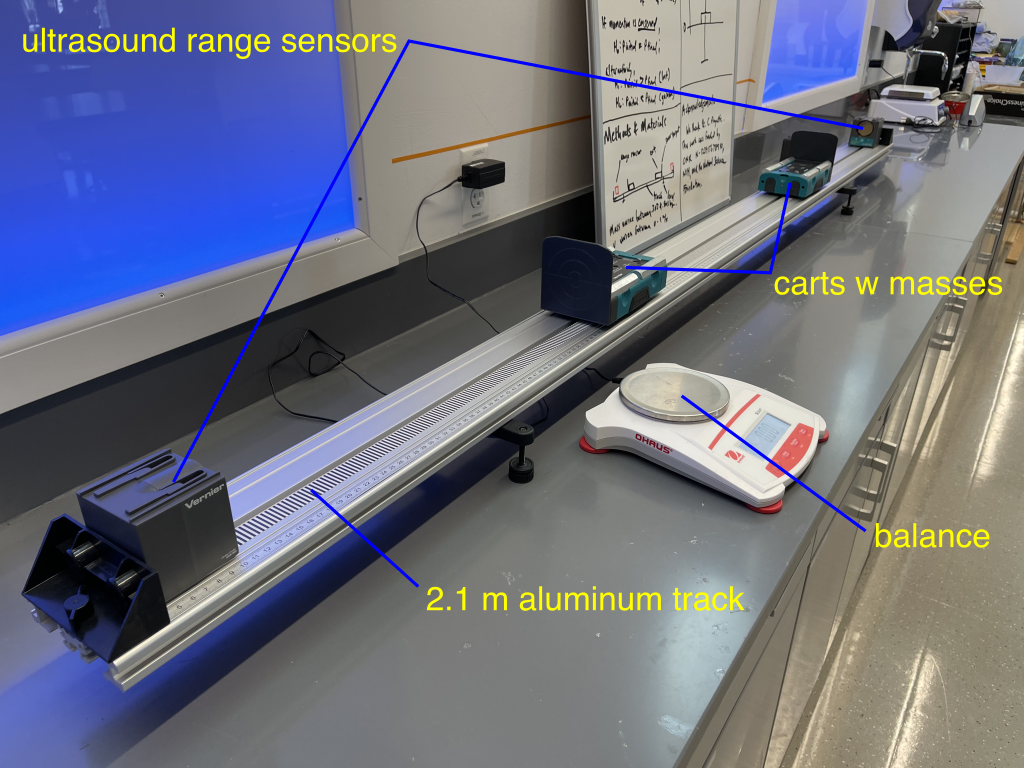
\includegraphics[width=\columnwidth]{fig1.png}
\end{center}
\caption{Momentum test track used for experiments. Total length \SI{2.1}{\meter}.}
\label{fig:methods1}
\end{figure}

\section{Methods and materials}
\subsection{Inelastic collision tests}
Inelastic collision tests ($n=72$) were conducted using a \SI{2.1}{\meter} aluminum momentum test track (Vernier; Beaverton, OR; see \fref{fig:methods1}). The test track was outfitted with two small wheeled carts (mass of cart \SI{0.3}{\kilo\gram}) with simple sliding contact bearings; mass of each cart could be increased by addition of up to four \SI{0.125}{\kilo\gram} masses for a total mass of \SI{0.8}{\kilo\gram}. The mass was measured using an electronic balance (Ohaus; Parsippany, NJ).    Magnets of opposite polarity allowed the carts to stick after the inelastic collision. Carts were actuated by hand to provide initial velocities. The position of the two carts was measured using two ultrasound range sensors (Go Direct; Vernier; Beaverton, OR). Sensor data were logged at \SI{20}{\hertz} sampling frequency, via a wireless Bluetooth link, using the Graphical Analysis app (Vernier; Beaverton, OR) running on an iPad Air (Apple; Cupertino, CA). From the position data, the slope of position versus time was used to estimate velocities before and after the collision.  A full factorial design was used to provide three replicates each for low and high levels of $m_1$, $m_2$, $v_1$, and three levels (stationary, towards, and away) of $v_2$.  

 \subsection{Momentum calculations}
 Calculations were performed using both Graphical Analysis and Sheets (Google; Mountain View, CA). 
 Momentum before the collision was calculated as
 \begin{equation}
 p_0 = m_1 v_1 + m_2 v_2.
 \end{equation}
Similarly, the final momentum was calculated as
 \begin{equation}
 p_f = m_1 v_{1,f} + m_2 v_{2,f}, 
 \end{equation}
and the difference in momentum as 
 \begin{equation}
\Delta p =  p_f - p_0. 
 \end{equation}
For nondimensional comparisons, we also computed the ratio of the masses ($\hat{\pi}_1=\frac{m_2}{m_1}$), the ratio of the velocities ($\hat{\pi}_2=\frac{v_2}{v_1}$), and the nondimensionalized change in momentum ($\Delta\hat{p}=\frac{\Delta p}{m_1 v_1}$). Additional plots and $t$-tests were done using R \cite{r-2021} and the \lstinline{tidyverse} library \cite{wickham-2019-welcome}. 

\section{Results}
%\subsection{Collision tests}
\Fref{fig:results1} shows the position data for a typical inelastic collision with equal masses, $m_1=m_2=\SI{0.3}{\kilo\gram}$. Before the collision, $m_2$ is stationary while $m_1$ approaches with velocity $v_1=\SI{0.62}{\meter\per\second}$. The masses collide at $t=\SI{1.5}{\second}$. After the collision, $m_1$ and $m_2$ are both moving with velocity $v_f=\SI{0.3}{\meter\per\second}$. 
\begin{figure}
\begin{center}
\includegraphics{inelastic.pdf}
\end{center}
\caption{Position data for a typical inelastic collision with equal masses, $m_1=m_2=\SI{0.3}{\kilo\gram}$. Initially, $m_2$ is stationary and $m_1$ is moving at \SI{0.62}{\meter\per\second}. The masses collide at $t=\SI{1.5}{\second}$. After the collision, $m_1$ and $m_2$ are both moving with velocity $v_f=\SI{0.3}{\meter\per\second}$. }
\label{fig:results1}
\end{figure}
%\subsection{Momentum calculations}
\Fref{fig:results2} shows a bar plot of the change in momentum during all collisions, $\Delta p = \SI{-0.01\pm0.06}{\kilo\gram\meter\per\second}$ (mean $\pm$ s.d.). The mean $\Delta p$ is not significantly different from \SI{0}{\kilo\gram\meter\per\second} (one-sample $t$-test, $n=72$, d.f.=71, $p=0.2596$). 
\begin{figure}
\begin{center}
\includegraphics{momentum-change.pdf}
\end{center}
\caption{Change in momentum ($\Delta p$) during all inelastic collisions. $\Delta p = \SI{-0.01\pm0.06}{\kilo\gram\meter\per\second}$ (mean $\pm$ s.d.). The mean $\Delta p$ is not significantly different from \SI{0}{\kilo\gram\meter\per\second} (one-sample $t$-test, $n=72$, d.f.=71, $p=0.2596$).}
\label{fig:results2}
\end{figure}

\section{Discussion}
\subsection{Is momentum conserved?}
\textbf{You will write this DISCUSSION paragraph \#1, which should also refer to \fref{fig:results2}.  Were any of the hypotheses supported? Were any refuted with the observed data? Based on your observations, is momentum conserved, or is it gained, or lost, during the collisions you have tested? What does it mean, big picture?}

\subsection{Sources of experimental error}
\textbf{You will write this DISCUSSION paragraph \#2. Please explain any limitations of the experiment, sources of experimental error, or things that should be taken into account when gauging the validity and applicability of your findings.}

\section{Acknowledgements}
We thank C.~Payette, J.~Bartholomew, B.~Turner, and S.~McCormick for useful advice and comments on the manuscript, and A.~Hahn and S.~Kealy for advice on the design of experiment and learning objectives. Major lab equipment was gifted by the Alumni Association at Morristown-Beard School. This work was funded by ONR \#N123456789, AFOSR, NIH, and the National Science Foundation. 

\bibliographystyle{apsrev4-1} % Tell bibtex which bibliography style to use
\bibliography{momentum} % Tell bibtex which .bib file to use (this one is some example file in TexLive's file tree)

\end{document}